\section{Results}
\label{sec:results}
Resultater vi mangler
\begin{itemize}
\item Franke - Bias varianse for Ridge og Lasso
\item Terrengdata - OLS
\item Terrengdata - Ridge
\item Terrengdata - Lasso
\item tabell minste feil for de ulike metodene (hvilken deg og $\lambda$)
\end{itemize}
\subsection{Regression on Franke's function}
The {''}terrain'' data $z$ in this part was produced by applying Franke's function to a $n\cross n$ evenly spaced $xy$ grid, with $x_i,y_i\in [0,1]$, and for each point added a normally distributed noise with $\mu = 0$ and $\sigma = 0.1$.
\subsubsection{$\beta$-values confidence interval}
Before applying any resampling methods we used the regular \emph{ordinary least squares} method \eqref{eq:ols} to our data and had a look at the confidence interval of the $\beta$ values when approximating the data to a polynomial of degree $m=5$. The confidence intervals are shown in Figure \ref{fig:betaconfidence}.
They range between 0.23 and 35 in width.  
\begin{figure}[htbp]
	\centering
	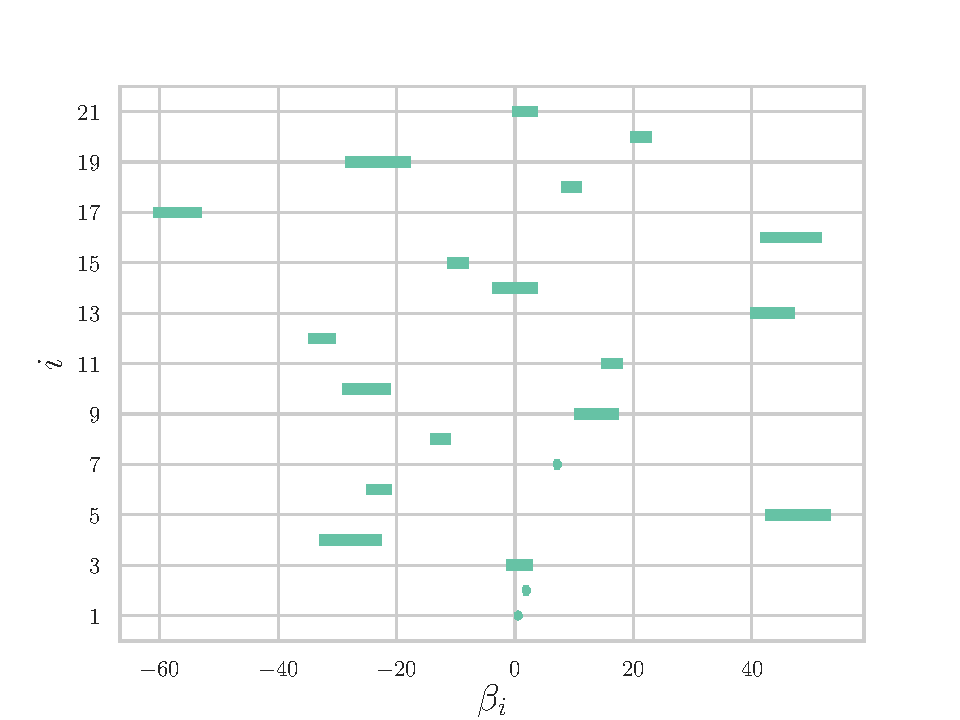
\includegraphics[width=0.5\textwidth]{betaconfidence}
	\caption{The $\beta$-values and their 95\% confidence interval with $m=5$ and $\sigma=0.1$ for OLS.}
	\label{fig:betaconfidence}
\end{figure}

\subsubsection{MSE and $R^2$ of OLS, with and without resampling}
To study the mean squared error \eqref{eq:mse} as a function of the model complexity, we applied the OLS-method to the data set for various values of polynomial degree $m$, both when using the entire data set as both test and training data, and by using the bootstrap method (Algorithm \ref{alg:bootstrap}) for resampling (Figure \ref{fig:mseVSdegreeOLS}).

% Eksempel for figurer
\begin{figure}[htbp]
	\centering
	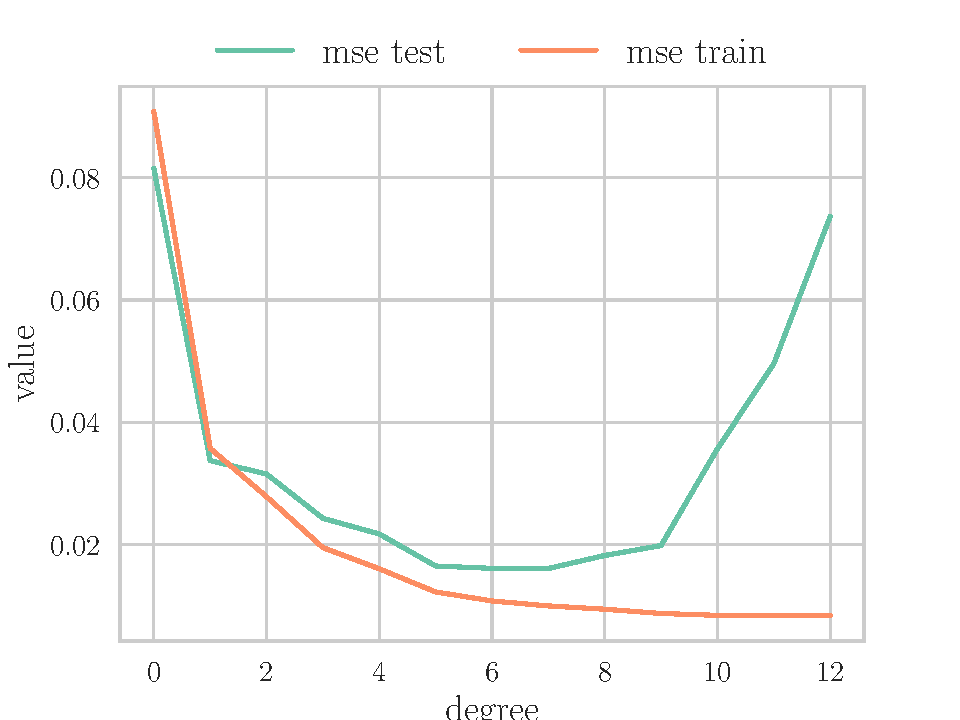
\includegraphics[width=0.5\textwidth]{mseVSdegreeOLS}
	\caption{MSE of the model as a function of degree $m$, with n=20, noise $\sigma$ = 0.1. In the case where no resampling is done (MSE-train), the MSE flattens out at a low value. When applying the bootstrap method (MSE-test) for resampling however, the MSE begins to rise after reaching a certain model complexity, creating a minimum point where the error is the lowest.}
	\label{fig:mseVSdegreeOLS}
\end{figure}

Applying the same analisys to the $R^2$-score \eqref{eq:r2} of the two cases, we get the result as shown in Figure \ref{fig:r2VSdegreeOLS}. For the $R^2$ score, we found the results easier to obtain when using the \emph{k-fold cross validation} method (Algorithm \ref{alg:k-fold}).
\begin{figure}[htbp]
	\centering
	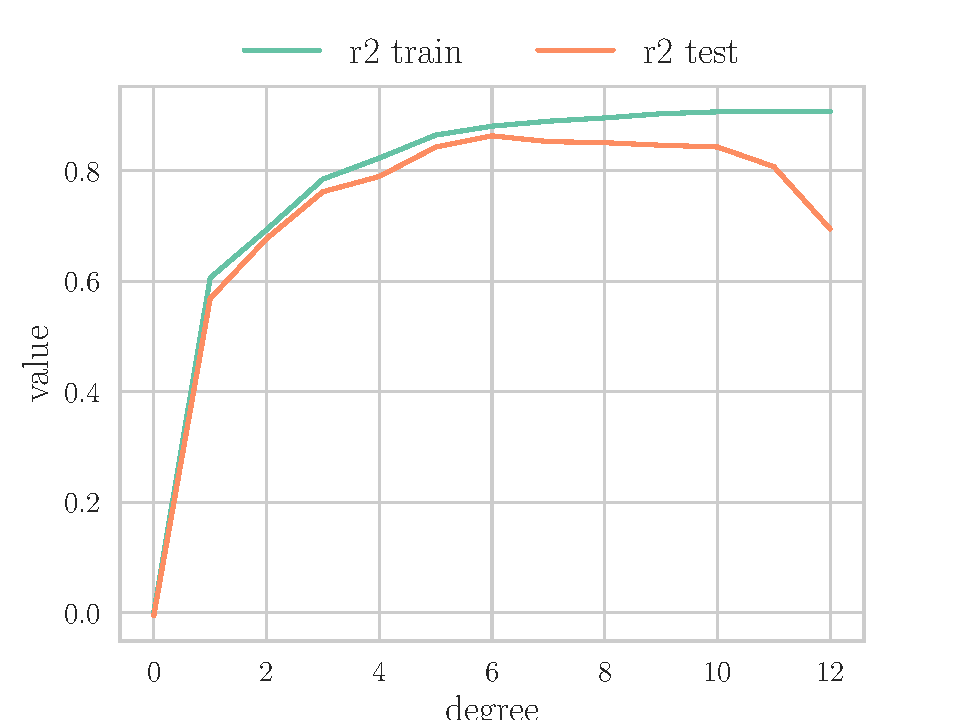
\includegraphics[width=0.5\textwidth]{r2VSdegreeOLS}
	\caption{$R^2$-score of the model as a function of degree $m$, with n=20, noise $\sigma$ = 0.1. In the case where no resampling is done (R2-train), the $R^2$ increases and then flattens out. When applying the k-fold cross validation method (R2-test) for resampling however, the $R^2$ begins to decrease after reaching a certain model complexity, creating a maximum point where the $R^2$-score is closest to 1 (the optimal value).}
	\label{fig:r2VSdegreeOLS}
\end{figure}

\subsubsection{Bias-Variance-tradeoff}
Sticking to the bootstrap method for resampling, and using $n=20$ with $\sigma = 0.1$ we also compute the bias and variance of the model as discussed in the theory. Plotting the variance, bias and MSE together results in Figure \ref{fig:biasvarianceOLS}.

\begin{figure}[htbp]
	\centering
	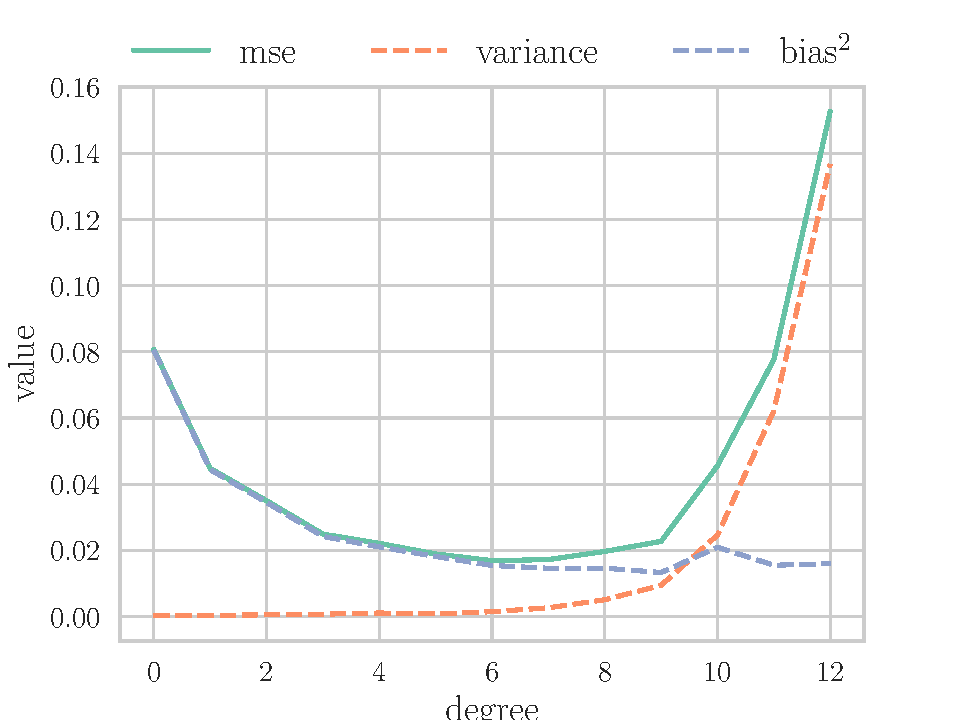
\includegraphics[width=0.5\textwidth]{biasvarianceOLS}
	\caption{Bias, variance and MSE for the ordinary least square method on the data set with $n=20$ and noise $\sigma=0.1$, resampled with the bootstrap method, as a function of model complexity/polynomial degree. The bias starts of high and decreases as the model complexity increases, whilst the variance grows with the model complexity.}
	\label{fig:biasvarianceOLS}
\end{figure}

\subsubsection{Resampling with Ridge-regression}
In order to find the parameters that will give the least MSE for the Ridge regression method, we need to tune both the degree $m$ of the polynomial that we fit, and the optimal $\lambda$-value. This is obtained by doing Ridge regression on the data set with bootstrap, for both different values of $m$ and different values of $\lambda$ as shown in Figure \ref{fig:lambdavsdegreesRIDGE}.

\begin{figure}[htbp]
	\centering
	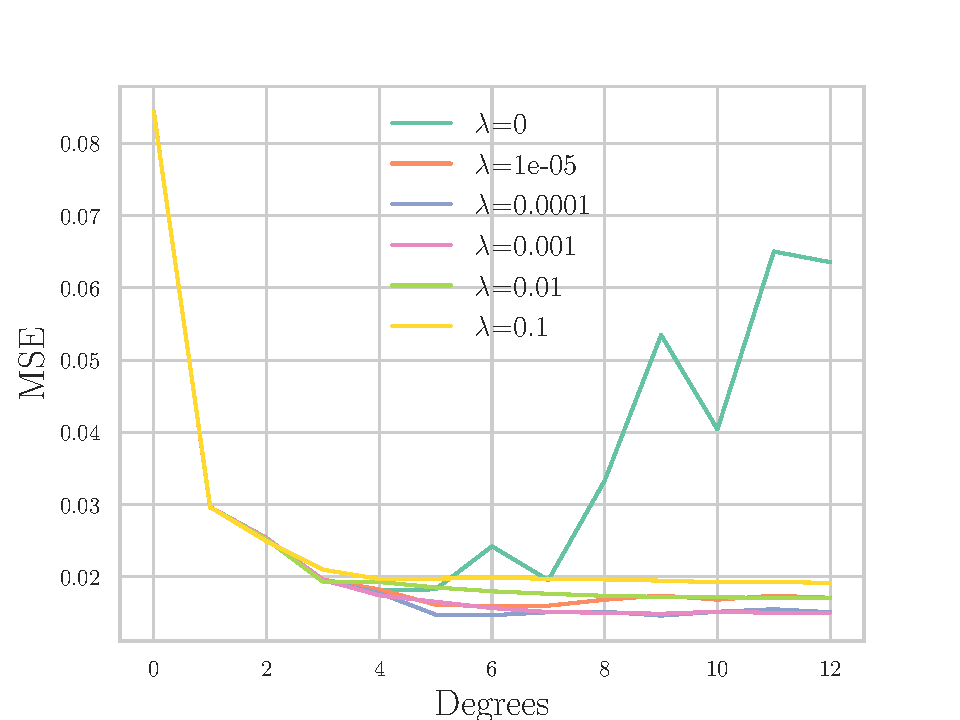
\includegraphics[width=0.5\textwidth]{lambdavsdegreesRIDGE}
	\caption{MSE for the Ridge regression method on the data set with $n=20$ and noise $\sigma=0.1$, resampled with the bootstrap method, as a function of model complexity/polynomial degree. The different lines in the plot represent different values of the hyperparameter $\lambda$. When $\lambda=0$ it is equivalent to the OLS-method.}
	\label{fig:lambdavsdegreesRIDGE}
\end{figure}

\subsubsection{Resampling with Lasso-regression}
The same analisys, with various $\lambda$ and $m$-values is done for Lasso-regression (Figure \ref{fig:lambdavsdegreesLASSO}).
\begin{figure}[htbp]
	\centering
	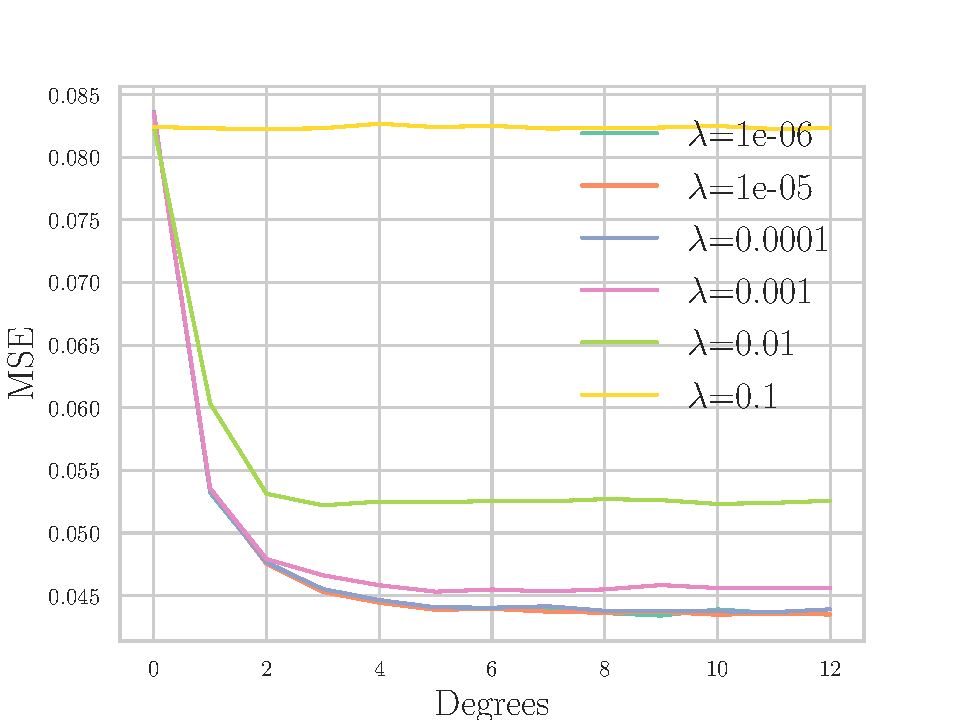
\includegraphics[width=0.5\textwidth]{lambdavsdegreesLASSO}
	\caption{MSE for the Lasso regression method on the data set with $n=20$ and noise $\sigma=0.1$, resampled with the bootstrap method, as a function of model complexity/polynomial degree. The different lines in the plot represent different values of the hyperparameter $\lambda$}
	\label{fig:lambdavsdegreesLASSO}
\end{figure}

\subsubsection{Comparing MSE of the different regression methods}
A different, and less visual way of finding the method that gives the best approximation, that is, the smallest MSE, is to store all the MSE data for all hyperparameters and degrees, make the computer find the smallest value, and the corresponding parameters which is presented in table \ref{tab:minerrorFRANKE}.
\begin{table}[htbp]
\caption{The smalles MSE for the different regressions methods, and the hyperparameter $\lambda$ and the degree $m$ that results the MSE in question. Produced using the bootstrap resampling method.}
\centering
\begin{tabular}[width=0.5\textwidth]{lccc}
\hline
\textbf{Reg} & \textbf{min. MSE} & $\boldsymbol{m}$ & $\boldsymbol{\lambda}$ \\
\hline
\textbf{OLS} & 0.016 & 7 & - \\
\textbf{Ridge} & 0.014 & 9 & 1e-05 \\
\textbf{Lasso} & 0.043 & 9 & 1e-06
\end{tabular}
\label{tab:minerrorFRANKE}
\end{table}

\subsubsection{Terrain data}

\begin{figure}[htbp]
	\centering
	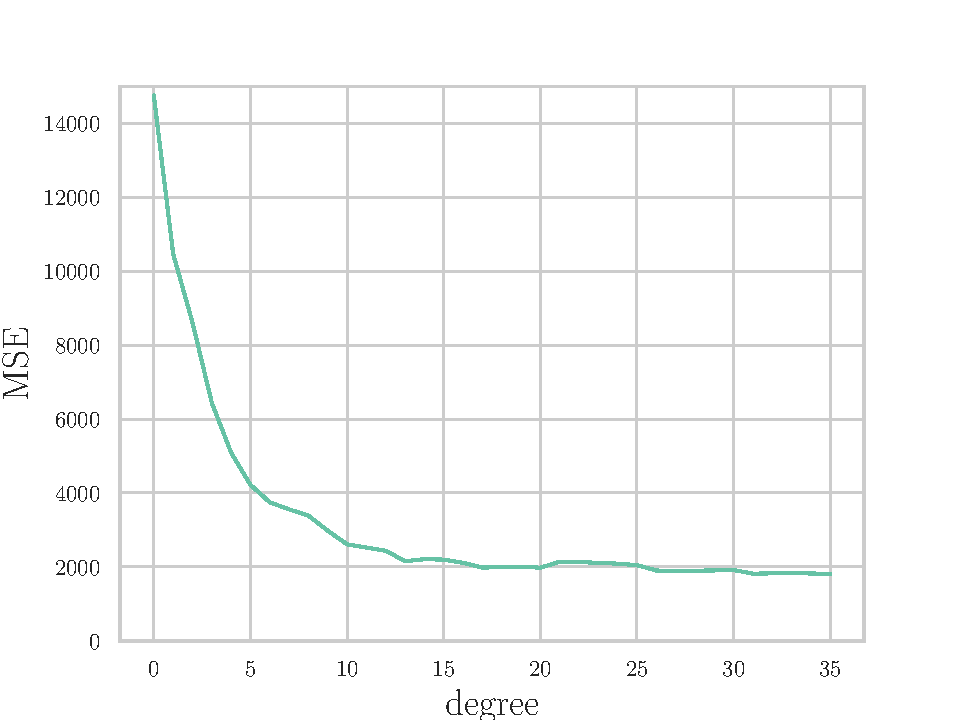
\includegraphics[width=0.5\textwidth]{mseVSdegreeOLS_terrain}
	\caption{MSE for the OLS regression method on the terrain data set.}
	\label{fig:mseVSdegreeOLSterrain}
\end{figure}

\vfill
\newpage
